\documentclass[11pt,a4paper]{article}

\usepackage{fontspec}
\usepackage{polyglossia}
\setmainlanguage{russian}
\setotherlanguage{english}
\IfFontExistsTF{Times New Roman}{\setmainfont{Times New Roman}}{\setmainfont{Libertinus Serif}}
\IfFontExistsTF{Menlo}{\newfontfamily\cyrillicfonttt{Menlo}}{\newfontfamily\cyrillicfonttt{DejaVu Sans Mono}}
\usepackage[a4paper,top=2.0cm,bottom=2.0cm,left=2.1cm,right=2.1cm]{geometry}
\usepackage{amsmath}
\usepackage{amssymb}
\usepackage{booktabs}
\usepackage{caption}
\usepackage{float}
\usepackage{graphicx}
\usepackage{hyperref}
\usepackage{xurl}
\usepackage{enumitem}
\usepackage{csquotes}
\usepackage{setspace}
\usepackage{array}

\hypersetup{
  colorlinks=true,
  linkcolor=black,
  citecolor=black,
  urlcolor=blue
}

\graphicspath{{../outputs/proposal_eda/}}
\setlength{\parindent}{1.25em}
\setlength{\parskip}{0.25em}
\setlist[itemize]{topsep=2pt,itemsep=2pt,parsep=0pt,leftmargin=1.6em}
\setlist[enumerate]{topsep=2pt,itemsep=2pt,parsep=0pt,leftmargin=1.8em}
\captionsetup{font=small,labelfont=bf}
\linespread{1.05}

\title{Эмпирическая оценка влияния загрязнения воздуха на ожидаемую продолжительность жизни в регионах Российской Федерации}
\author{Ковалёва М.\,С., Кутузов И.\,В., Николюк Т.\,Н.}
\date{Москва, 2026}

\documentclass[10pt,a4paper]{article}

\usepackage{fontspec}
\usepackage{polyglossia}
\setmainlanguage{russian}
\setotherlanguage{english}
\defaultfontfeatures{Ligatures=TeX}
\setmainfont{LinLibertine_R.otf}[
  BoldFont       = LinLibertine_RB.otf,
  ItalicFont     = LinLibertine_RI.otf,
  BoldItalicFont = LinLibertine_RBI.otf
]
\newfontfamily\cyrillicfonttt{LinLibertine_R.otf}[
  BoldFont       = LinLibertine_RB.otf,
  ItalicFont     = LinLibertine_RI.otf,
  BoldItalicFont = LinLibertine_RBI.otf
]

\usepackage[a4paper,top=2.0cm,bottom=2.0cm,left=2.1cm,right=2.1cm]{geometry}
\usepackage{graphicx}
\usepackage{booktabs}
\usepackage{amsmath}
\usepackage{amssymb}
\usepackage{caption}
\usepackage{hyperref}
\usepackage{xurl}
\usepackage{csquotes}
\usepackage{enumitem}
\usepackage{setspace}
\usepackage[round,authoryear]{natbib}
\usepackage{titlesec}
\usepackage{multicol}
\usepackage{float}

\titlespacing*{\section}{0pt}{1.2ex plus 0.3ex minus 0.2ex}{0.5ex plus 0.2ex}
\titlespacing*{\subsection}{0pt}{0.8ex plus 0.2ex minus 0.1ex}{0.3ex plus 0.1ex}
\titleformat*{\section}{\normalfont\Large\bfseries}
\titleformat*{\subsection}{\normalfont\large\bfseries}

\setlist[itemize]{topsep=2pt, partopsep=1pt, itemsep=2pt, parsep=0pt, leftmargin=1.6em}
\setlist[enumerate]{topsep=2pt, partopsep=1pt, itemsep=2pt, parsep=0pt, leftmargin=1.8em}

\setlength{\abovecaptionskip}{4pt}
\setlength{\belowcaptionskip}{2pt}
\setlength{\textfloatsep}{6pt plus 2pt minus 2pt}
\setlength{\intextsep}{6pt plus 2pt minus 2pt}
\setlength{\floatsep}{6pt plus 2pt minus 2pt}

\hypersetup{
  colorlinks=true,
  linkcolor=black,
  citecolor=black,
  urlcolor=blue
}

\graphicspath{{../outputs/proposal_eda/}}

\setlength{\parskip}{0.20em}
\setlength{\parindent}{1.25em}
\setlength{\emergencystretch}{3em}
\linespread{1.04}\selectfont
\setlength{\bibsep}{1pt plus 0.2ex}
\setlength{\abovedisplayskip}{3pt}
\setlength{\belowdisplayskip}{3pt}
\setlength{\abovedisplayshortskip}{2pt}
\setlength{\belowdisplayshortskip}{2pt}
\setlength{\jot}{2pt}

\title{Эмпирическая оценка влияния степени загрязнения воздуха на ожидаемую продолжительность жизни в регионах Российской Федерации}
\author{Ковалёва М.\,С., Кутузов И.\,В., Николюк Т.\,Н.}
\date{Москва, 2026}

\begin{document}

\begin{titlepage}
\centering
\vspace*{1cm}
{\large Федеральное государственное автономное образовательное учреждение\\
высшего образования\par}
\vspace{0.5cm}
{\Large \textbf{НАЦИОНАЛЬНЫЙ ИССЛЕДОВАТЕЛЬСКИЙ УНИВЕРСИТЕТ}\par}
\vspace{0.3cm}
{\Large \textbf{<<ВЫСШАЯ ШКОЛА ЭКОНОМИКИ>>}\par}
\vspace{0.5cm}
{\large Факультет экономических наук\par}
\vspace{0.3cm}
{\large Эконометрика\par}

\vfill

{\Large\bfseries Эмпирическая оценка влияния степени загрязнения воздуха на ожидаемую продолжительность жизни в регионах Российской Федерации\par}

\vfill

\begin{flushright}
\begin{minipage}{0.6\textwidth}
\raggedleft
\textbf{Выполнили:}\\[0.3em]
Ковалёва Мария Сергеевна\\
Кутузов Иван Владимирович\\
Николюк Татьяна Николаевна\\[1em]
\textbf{Преподаватель семинаров:}\\[0.3em]
Бывальцева-Станкевич\\
Анастасия Александровна
\end{minipage}
\end{flushright}

\vfill
{\large г.~Москва, 2026 г.\par}
\end{titlepage}

\section*{Введение}

Загрязнение атмосферного воздуха~--- одна из наиболее значимых экологических и социально-экономических проблем современности. По оценкам Всемирной организации здравоохранения, загрязнение воздуха связано с повышенным риском сердечно-сосудистых, респираторных и онкологических заболеваний, что непосредственно негативно влияет на качество и ожидаемую продолжительность жизни. Для России данная проблема вызывает особый интерес вследствие высокой неоднородности регионов по уровню промышленной нагрузки, энергетической структуры экономики и концентрации вредных выбросов. В ряде субъектов РФ сохраняется высокий уровень загрязнения атмосферы, связанный с деятельностью металлургии, теплоэнергетики, добывающей промышленности и тяжёлого производства.

\medskip

Таким образом, становится важным в рамках данного исследования определить влияние загрязнения воздуха на ожидаемую продолжительность жизни в регионах РФ для возможной корректировки политики в сторону улучшения экологической обстановки, а также повышения осведомлённости населения об угрозе для жизни в их регионе, представленной высокой концентрацией токсичных веществ в атмосферном воздухе.

\section*{Цель исследования}

Цель данного эмпирического исследования~--- оценка статистической значимости, силы и направления влияния степени загрязнения воздуха на ожидаемую продолжительность жизни населения по субъектам РФ.

Дополнительно исследование направлено на:
\begin{itemize}
  \item выявление факторов, которые являются причиной региональных различий в продолжительности жизни;
  \item проверку наличия эндогенности между загрязнением и иными характеристиками регионов;
  \item оценку применимости инструментальных переменных для идентификации и борьбы с эндогенностью.
\end{itemize}

\section*{Актуальность исследования}

Высокий риск смертности, связанный с сильным загрязнением воздуха, остаётся актуальной проблемой во всём мире. Это подтверждается ежегодными отчётами <<State of Global Air>> от исследовательских организаций Health Effects Institute и Institute for Health Metrics and Evaluation. Так, например, в отчёте на 2025~г. подчёркивается, что загрязнение воздуха остаётся вторым ведущим риск-фактором ранней смерти, уступая только высокому кровяному давлению. Кроме того, в 2023 году во всём мире 7{,}9~млн смертей были связаны с загрязнением атмосферы, которое включает в себя концентрацию $\text{PM}_{2.5}$ (микрочастиц), загрязнение воздуха домашних хозяйств и воздействие озона, содержание которого сейчас на 30--70\% выше, чем 100 лет назад. В глобальном распределении смертности, связанной с загрязнением воздуха, центральная и восточная Европа вместе с центральной Азией занимают 4{,}5\%, что невелико в сравнении с югом и востоком Азии и Океанией (в совокупности 68{,}2\%), но по-прежнему значимо в рамках региональной проблемы.

\medskip

Важность проблемы мирового загрязнения воздуха подчёркивается также и в отчёте Института энергетической политики Чикагского университета <<Air Quality Life Index Annual Update>> 2025~г., в котором отмечается, что в 2023~г. глобальная концентрация $\text{PM}_{2.5}$ повысилась на 1{,}5\% в сравнении с 2022~г. и почти в 5 раз превысила рекомендуемый ВОЗ уровень в 5~мкг/м³, достижение которого обеспечило бы повышение средней продолжительности жизни примерно на 1{,}9 лет, что в общей сложности увеличило бы численность населения планеты на 15{,}1~млрд лет. Таким образом, отчёт напрямую интерпретирует загрязнение воздуха через потери ожидаемой продолжительности жизни, что соответствует логике настоящего исследования. Также он повествует и о положительных изменениях в экологической политике стран, направленной на снижение атмосферного загрязнения~--- например, о введении Евросоюзом в 2024~г. ограничения на концентрацию $\text{PM}_{2.5}$ в 10~мкг/м³ до конца 2030~г., что безусловно влияет на увеличение средней продолжительности жизни.

\medskip

Связь смертности и загрязнения воздуха в России была описана уже более 25 лет назад в работе Б.\,А. Ревича и А.\,А. Быкова (1998~г.), в которой констатировалась 7\%-я смертность от загрязнения воздуха только взвешенными веществами для населения в 15~млн. Кроме того, авторы призывают к детальному рассмотрению этой темы и новым исследованиям.

Немаловажной в рамках темы является статья V.\,P. Reshetin, V.\,I. Kazazyan (2004~г.) <<Public-Health Impact of Outdoor Air Pollution in Russia>>, основой которой послужили данные мониторинга Росгидромета за 1993 и 1998 годы. По их расчётам, загрязнение воздуха частицами может быть связано с 219--233~тыс. преждевременных смертей или 15--17\% смертности в год. Авторы подчёркивают необходимость внедрения мер по снижению экологических рисков в городах РФ.

\medskip

С 2018~г. в стране действует национальный проект <<Чистый воздух>>, направленный на снижение выбросов в 12 наиболее загрязнённых городах. Но несмотря на всю практическую значимость проблемы, эконометрическая литература по причинному эффекту загрязнения на продолжительность жизни на российских данных остаётся крайне ограниченной, что подчёркивает необходимость проведения исследования.

\section*{Гипотезы исследования}

\textbf{Гипотеза 1. Рост выбросов загрязняющих веществ на душу населения сокращает ожидаемую продолжительность жизни в регионах РФ.}
\begin{align*}
H_0\colon\ & \beta_1 = 0 \quad \text{(выбросы не влияют на ОПЖ)}\\
H_1\colon\ & \beta_1 < 0 \quad \text{(рост выбросов сокращает ОПЖ)}
\end{align*}
Ожидаемое направление: $\beta_1 < 0$ в спецификации (\ref{eq:ss}).

В обоснование гипотезы можно привести несколько работ. Pope et al. (2002) показали на данных American Cancer Society, что рост долгосрочной концентрации $\text{PM}_{2.5}$ на 10~мкг/м³ увеличивает сердечно-сосудистую и лёгочную смертность примерно на 6\% и 8\%. Chen et al. (2013) и Ebenstein et al. (2017) на данных о реке Хуайхэ оценили потери продолжительности жизни на севере Китая (с большей концентрацией выбросов) в 3--5 лет. Currie \& Neidell (2005) добавляют, что значимые эффекты на здоровье фиксируются даже при относительно невысоких уровнях экспозиции (низких уровнях загрязнения воздуха). Наконец, Ревич и Быков (1998) оценили избыточную смертность от атмосферных выбросов непосредственно для крупных городов России.

\textbf{Гипотеза 2. После контроля на загрязнение и возрастную структуру доход положительно связан с ОПЖ.}
\begin{align*}
H_0\colon\ & \beta_{\text{grp\_pc}} = 0 \quad \text{(доход не связан с ОПЖ при прочих равных)}\\
H_1\colon\ & \beta_{\text{grp\_pc}} > 0 \quad \text{(более богатые регионы живут дольше при фиксированном уровне загрязнения)}
\end{align*}

Preston (1975) показал устойчивую положительную связь между национальным доходом на душу населения и ОПЖ в межстрановом разрезе, однако подчеркнул, что значительная часть вариации определяется факторами, экзогенными доходу. В российских регионах сырая корреляция отрицательна ($r = -0{,}13$), что отражает специфику сырьевых территорий: высокий ВРП здесь сопряжён с промышленной нагрузкой, суровым климатом и специфической структурой занятости, а не с теми механизмами улучшения здоровья, которые описывает Preston. Соответственно, ожидается, что $\hat\beta_{\text{grp\_pc}} > 0$. Это подчёркивает необходимость явного контроля дохода (отдельный регрессор).

\textbf{Гипотеза 3. Занятость в добыче полезных ископаемых на душу населения связана с уровнем загрязнения воздуха после учёта контрольных переменных.}
\begin{align*}
H_0\colon\ & \pi_1 = 0\\
H_1\colon\ & \pi_1 > 0
\end{align*}

Проверка релевантности~--- необходимое условие 2SLS. Добыча~--- отрасль с высокой эмиссионной интенсивностью на занятого (в связи с чем ожидаем $\pi_1 > 0$). Greenstone (2002) и Chay \& Greenstone (2003) показали, что отраслевая структура региона по американским данным~--- один из главных экзогенных факторов локального уровня загрязнения.

\section*{Данные}

В работе были использованы кросс-секционные данные по 85 регионам России за 2015 год, так как именно за этот год данные имелись в наиболее полном объёме. Основной источник данных~--- Fedstat, ссылки на конкретные датасеты представлены в приложении. Все переменные, описанные ниже, являются непрерывными количественными. Также используется переменная \texttt{region}~--- категориальная. В моделях используются логарифмы некоторых переменных.

\textbf{Зависимая переменная.} \texttt{life\_expectancy}~--- ожидаемая продолжительность жизни в годах, основной показатель здоровья населения.

\textbf{Основная объясняющая переменная.} \texttt{emissions\_h1\_pc}~--- выбросы загрязняющих веществ от стационарных источников на душу населения, тыс.~тонн на человека.

\textbf{Инструментальные переменные:}
\begin{itemize}
  \item \texttt{emp\_mining\_pc}~--- занятость в добыче полезных ископаемых на душу населения, основной инструмент;
  \item \texttt{emissions\_fuel\_pc}~--- выбросы от сжигания топлива на душу населения;
  \item \texttt{emp\_energy\_pc}~--- занятость в энергетике на душу населения.
\end{itemize}

\textbf{Контрольные переменные:}
\begin{itemize}
  \item \texttt{grp\_pc}~--- ВРП на душу населения, тыс.~руб. на человека;
  \item \texttt{urban\_share}~--- доля городского населения;
  \item \texttt{age\_struct\_share}~--- доля населения старших возрастов;
  \item \texttt{population\_avg}~--- среднегодовая численность населения, человек.
\end{itemize}

\textbf{Дополнительные переменные:}
\begin{itemize}
  \item \texttt{industrial\_index}~--- индекс промышленного производства;
  \item \texttt{visits\_per\_capita}~--- число посещений лечебных учреждений на одного жителя;
  \item \texttt{emp\_manufacturing\_pc}~--- занятость в обрабатывающих производствах на душу населения;
  \item \texttt{emp\_construction\_pc}~--- занятость в строительстве на душу населения;
  \item \texttt{emp\_metallurgy\_pc}~--- занятость в металлургии на душу населения;
  \item \texttt{emp\_chemicals\_pc}~--- занятость в химическом производстве на душу населения.
\end{itemize}

\section*{Методы и спецификация модели}

Оценивание проводится в два шага. Сначала строится базовая OLS-регрессия~--- она даёт состоятельные оценки только при отсутствии эндогенности, которая здесь может присутствовать. Затем применяется 2SLS, где в качестве инструмента для эндогенной переменной \texttt{ln\_emissions\_h1\_pc} выступает логарифм занятости в добыче полезных ископаемых на душу населения. Во всех спецификациях стандартные ошибки скорректированы на гетероскедастичность (HC1).

Базовая OLS-регрессия (уравнение 1):
\begin{equation}
\label{eq:ols}
\begin{aligned}
\text{life\_expectancy}_i = {} & \beta_0 + \beta_1\,\text{ln\_emissions\_h1\_pc}_i + \beta_2\,\text{ln\_grp\_pc}_i \\
& + \beta_3\,\text{urban\_share}_i + \beta_4\,\text{age\_struct\_share}_i \\
& + \beta_5\,\text{ln\_population\_avg}_i + \varepsilon_i
\end{aligned}
\end{equation}

Первая ступень 2SLS (уравнение 2):
\begin{equation}
\label{eq:fs}
\begin{aligned}
\text{ln\_emissions\_h1\_pc}_i = {} & \pi_0 + \pi_1\,\text{ln\_emp\_mining\_pc}_i + \pi_2\,\text{ln\_grp\_pc}_i \\
& + \pi_3\,\text{urban\_share}_i + \pi_4\,\text{age\_struct\_share}_i \\
& + \pi_5\,\text{ln\_population\_avg}_i + v_i
\end{aligned}
\end{equation}

Вторая ступень 2SLS (уравнение 3):
\begin{equation}
\label{eq:ss}
\begin{aligned}
\text{life\_expectancy}_i = {} & \beta_0 + \beta_1\,\widehat{\text{ln\_emissions\_h1\_pc}}_i + \beta_2\,\text{ln\_grp\_pc}_i \\
& + \beta_3\,\text{urban\_share}_i + \beta_4\,\text{age\_struct\_share}_i \\
& + \beta_5\,\text{ln\_population\_avg}_i + \varepsilon_i
\end{aligned}
\end{equation}

Логарифмическая форма для выбросов, ВРП и численности населения выбрана из-за правосторонней асимметрии этих переменных. Коэффициент $\beta_1$ интерпретируется как полу-эластичность: изменение ОПЖ в годах при удвоении выбросов на душу населения равно $\beta_1\cdot\ln 2 \approx \beta_1\cdot 0{,}693$.

\section*{Эндогенность и инструментальная стратегия}

OLS-оценка $\beta_1$ из уравнения~(\ref{eq:ols}) смещена как минимум в силу:
\begin{itemize}
  \item пропущенных переменных~--- качество здравоохранения, климат, исторически сложившаяся отраслевая структура связаны одновременно и с загрязнением, и с продолжительностью жизни;
  \item ошибок измерения в \texttt{emissions\_h1}, которая не учитывает транспорт, бытовое отопление и трансграничный перенос;
  \item миграционных причин~--- здоровые трудоспособные граждане концентрируются в индустриальных регионах, искусственно завышая там наблюдаемую продолжительность жизни.
\end{itemize}

Ожидается, что $|\hat\beta_{\text{2SLS}}| > |\hat\beta_{\text{OLS}}|$, что согласуется с направлением смещения, обсуждаемым выше.

В качестве инструмента используется логарифм занятости в добыче полезных ископаемых на душу населения. Его релевантность объясняется тем, что размещение добывающих производств определяется геологией и освоением территорий, а не текущей политикой здравоохранения, тогда как добыча и первичная переработка сырья~--- один из главных источников стационарных выбросов. Ожидается, что $F$-статистика первой ступени превысит порог Staiger \& Stock (1997) $F > 10$; в случае умеренной силы инструмента будут применены робастные к слабым инструментам методы.

\section*{Диагностика и робастность}

Планируется: (1) тест Wu--Hausman / Дурбина на экзогенность регрессора; (2) проверка силы инструмента по частной $F$-статистике с критическими значениями Stock \& Yogo (2005); (3) VIF-анализ мультиколлинеарности; (4) тест Саргана при использовании более одного инструмента; (5) переоценка без влиятельных наблюдений (Cook's distance, leverage); (6) альтернативные инструменты~--- занятость в энергетике.

\section*{Ограничения}

Кросс-секция за один год не позволяет контролировать ненаблюдаемую региональную гетерогенность через фиксированные эффекты~--- это недостаток, который лишь частично компенсирует инструментальная переменная. Данные об \texttt{emissions\_h1} охватывают только стационарные источники, исключая транспорт и бытовой сектор, что занижает суммарную экспозицию.

\section*{Предварительный анализ данных}

\begin{table}[H]
\centering
\caption{Дескриптивные статистики основных переменных}
\label{tab:desc}
\begin{tabular}{lrrrrr}
\toprule
\textbf{Переменная} & \textbf{Среднее} & \textbf{Ст.\,откл.} & \textbf{Мин} & \textbf{Медиана} & \textbf{Макс} \\
\midrule
\texttt{life\_expectancy}    & 70{,}5662  & 2{,}3977  & 63{,}1400   & 70{,}3900  & 78{,}4700 \\
\texttt{ln\_emissions\_h1\_pc} & $-10{,}3097$ & 1{,}4159 & $-14{,}5157$ & $-10{,}2621$ & $-6{,}9957$ \\
\texttt{ln\_emp\_mining\_pc}  & $-5{,}5818$  & 1{,}6311 & $-8{,}7341$  & $-5{,}9033$  & $-1{,}5898$ \\
\texttt{ln\_grp\_pc}          & 5{,}8500   & 0{,}6917  & 4{,}6834    & 5{,}7689   & 8{,}5867 \\
\texttt{urban\_share}        & 70{,}2682  & 13{,}2684 & 29{,}9000   & 71{,}4000  & 100{,}0000 \\
\texttt{age\_struct\_share}  & 58{,}2165  & 2{,}0328  & 54{,}2000   & 57{,}7000  & 64{,}9000 \\
\texttt{ln\_population\_avg} & 13{,}9713  & 0{,}9782  & 10{,}6546   & 13{,}9885  & 16{,}3233 \\
\bottomrule
\end{tabular}
\end{table}

\begin{figure}[H]
\centering
\begin{minipage}[t]{0.49\textwidth}
\centering
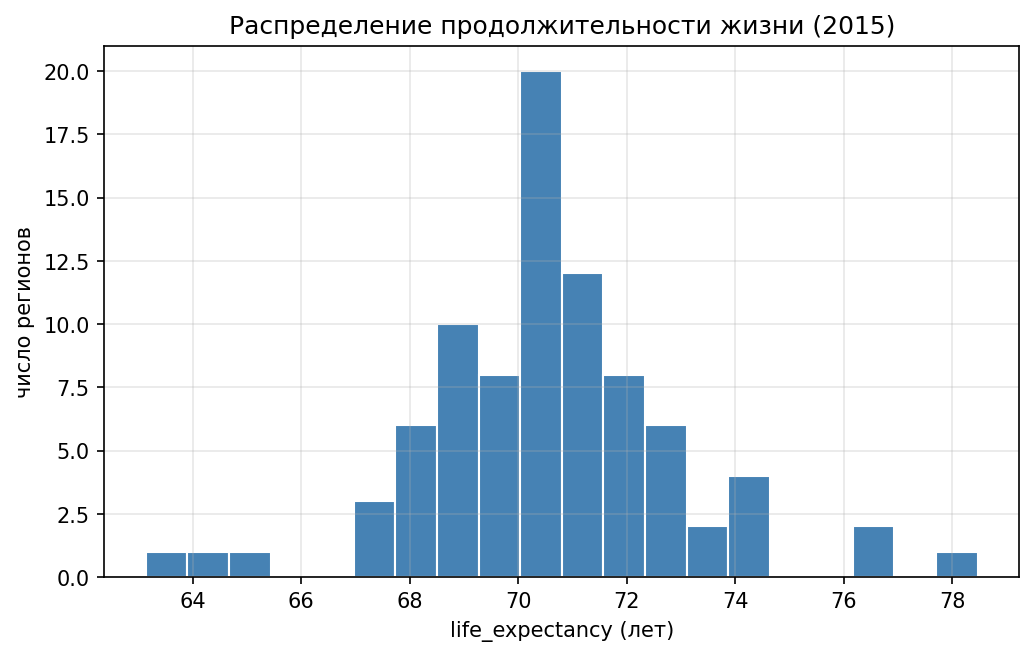
\includegraphics[width=\linewidth]{01_life_expectancy_distribution.png}
\caption{Распределение ожидаемой продолжительности жизни по регионам РФ}
\label{fig:le}
\end{minipage}\hfill
\begin{minipage}[t]{0.49\textwidth}
\centering
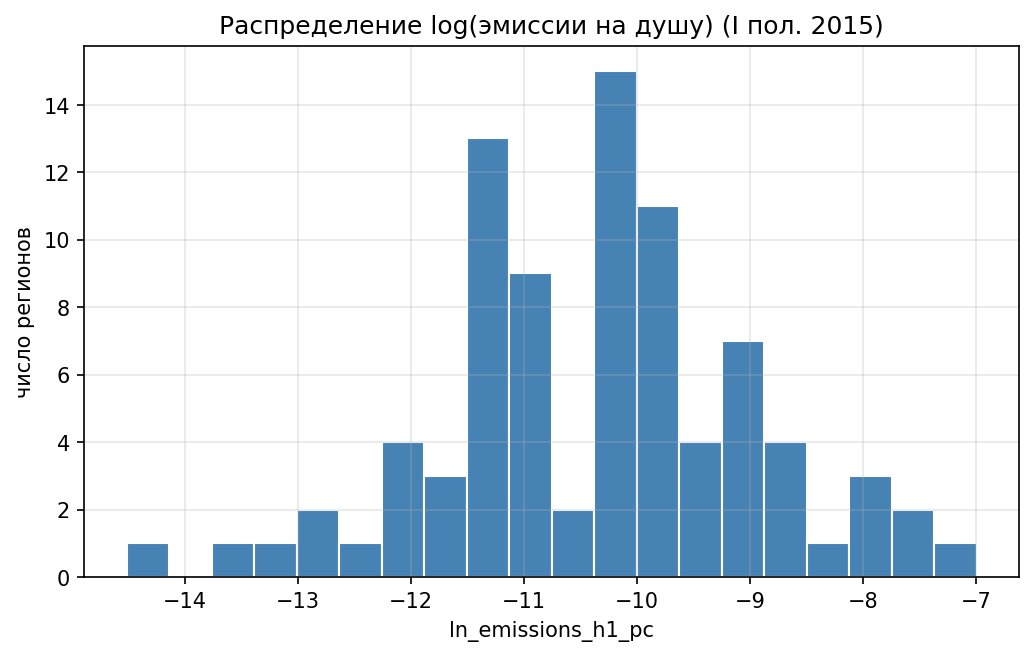
\includegraphics[width=\linewidth]{02_emissions_distribution.png}
\caption{Распределение логарифма выбросов загрязняющих веществ на душу населения}
\label{fig:em}
\end{minipage}
\end{figure}

\begin{figure}[H]
\centering
\begin{minipage}[t]{0.49\textwidth}
\centering
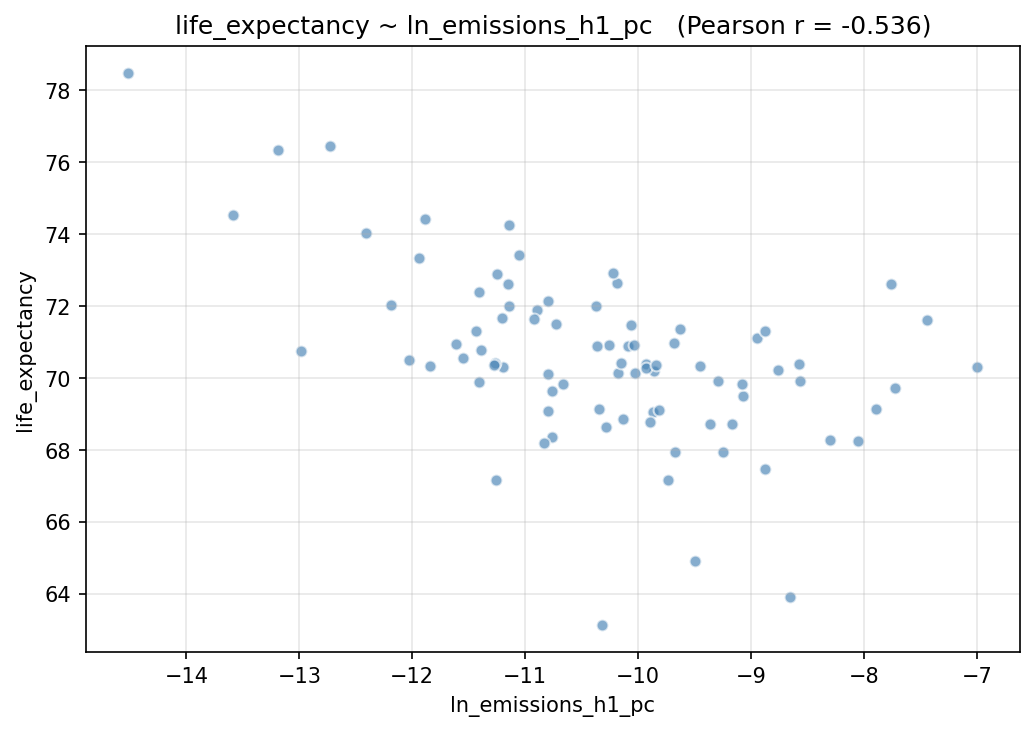
\includegraphics[width=\linewidth]{03_life_expectancy_vs_emissions.png}
\caption{Связь между загрязнением воздуха и ожидаемой продолжительностью жизни}
\label{fig:le_em}
\end{minipage}\hfill
\begin{minipage}[t]{0.49\textwidth}
\centering
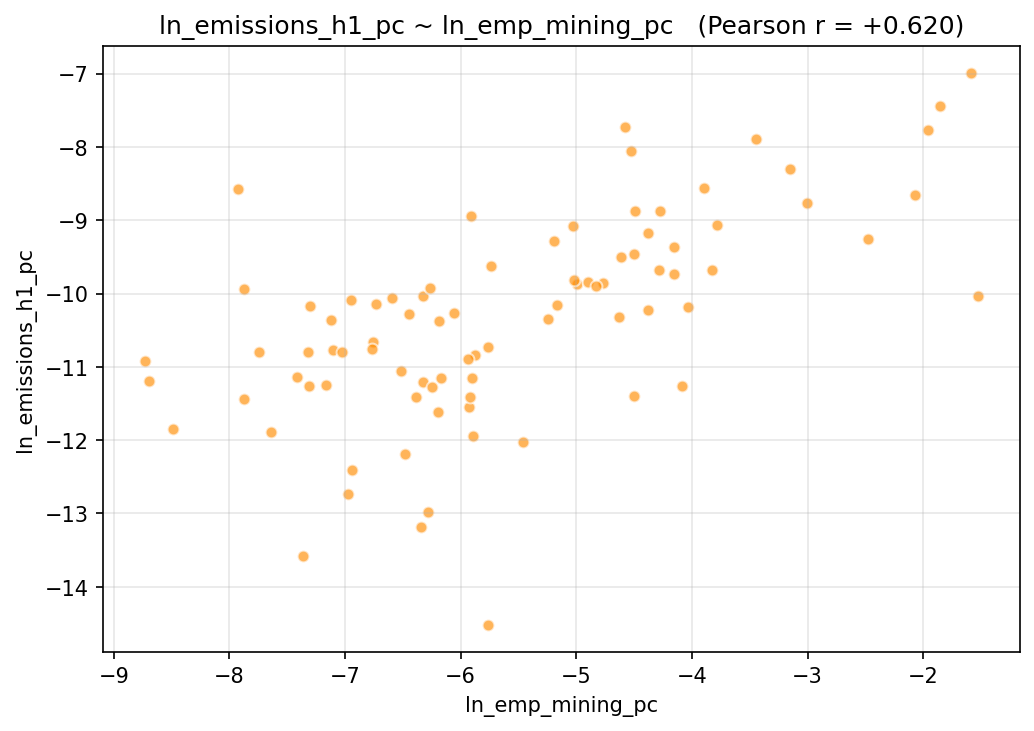
\includegraphics[width=\linewidth]{04_emissions_vs_mining_instrument.png}
\caption{Связь между занятостью в добыче полезных ископаемых и загрязнением воздуха}
\label{fig:em_mining}
\end{minipage}
\end{figure}

\begin{figure}[H]
\centering
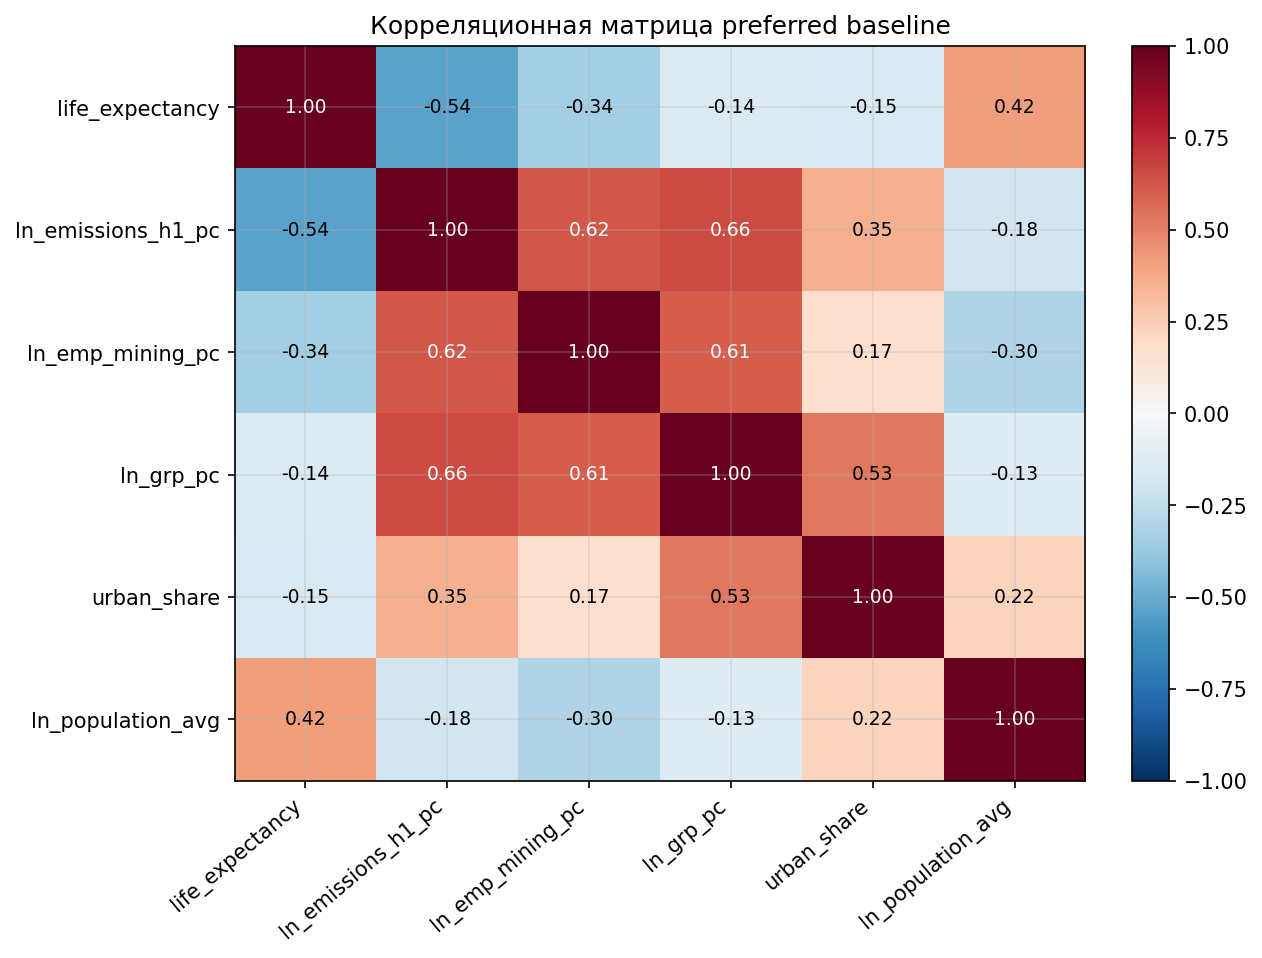
\includegraphics[width=0.55\textwidth]{05_correlation_heatmap.png}
\caption{Корреляционная матрица основных переменных}
\label{fig:corr}
\end{figure}

Предварительный анализ данных позволил сделать несколько содержательных выводов: по некоторым показателям, таким как загрязнение воздуха, значения существенно различаются, что объясняется тем, что в регионах разный уровень развития промышленности. Распределение выбросов заметно асимметрично, так что данная переменная обоснованно прологарифмирована. Между ОПЖ и загрязнением воздуха наблюдается умеренная отрицательная корреляция. Занятость в добыче положительно связана с загрязнением, что подтверждает релевантность инструмента.

\section{Данные и изменения после proposal}

Используются кросс-секционные данные по 85 субъектам РФ за 2015 год. Основной источник данных~--- Росстат/Fedstat. Зависимая переменная \texttt{life\_expectancy} измеряет ожидаемую продолжительность жизни в годах. Основная объясняющая переменная \texttt{ln\_emissions\_h1\_pc}~--- логарифм выбросов загрязняющих веществ от стационарных источников на душу населения. В качестве основного инструмента используется \texttt{ln\_emp\_mining\_pc}~--- логарифм занятости в добыче полезных ископаемых на душу населения.

В финальной версии были внесены три важных уточнения относительно proposal.

\begin{enumerate}
  \item \textbf{Проверка автономных округов.} В одной из промежуточных версий датасета Архангельская область и Тюменская область были записаны как региональные totals <<с АО>>, тогда как Ненецкий АО, Ханты-Мансийский АО и Ямало-Ненецкий АО также присутствовали отдельными строками. Это создавало риск двойного счёта. В финальном ноутбуке используется исправленная версия, где Архангельская область и Тюменская область берутся без автономных округов. Например, население Архангельской области в финальном датасете равно 1{,}094{,}549, а Тюменской области~--- 1{,}462{,}199; автономные округа остаются отдельными наблюдениями.
  \item \textbf{Возрастная структура.} \texttt{age\_struct\_share} не включается в preferred baseline, поскольку демографическая структура может быть outcome-related: высокая или низкая доля отдельных возрастных групп может отражать прошлую смертность, миграцию и региональную селекцию. Поэтому она используется только в robustness specification.
  \item \textbf{Обращаемость в медучреждения.} \texttt{visits\_per\_capita} не включается в baseline. Эта переменная может отражать не только доступность медицины, но и текущую заболеваемость, то есть сама быть связанной с результатом. Кроме того, как proxy качества здравоохранения она достаточно шумная.
\end{enumerate}

Переменная \texttt{region} используется только как идентификатор наблюдений и не включается в модели как категориальный регрессор.

\begin{table}[H]
\centering
\caption{Дескриптивные статистики основных переменных}
\label{tab:desc}
\begin{tabular}{lrrrrr}
\toprule
\textbf{Переменная} & \textbf{Среднее} & \textbf{Ст. откл.} & \textbf{Мин.} & \textbf{Медиана} & \textbf{Макс.} \\
\midrule
\texttt{life\_expectancy}       & 70{,}554 & 2{,}394 & 63{,}140 & 70{,}390 & 78{,}470 \\
\texttt{ln\_emissions\_h1\_pc}  & -10{,}336 & 1{,}393 & -14{,}516 & -10{,}262 & -6{,}996 \\
\texttt{ln\_emp\_mining\_pc}    & -5{,}571 & 1{,}655 & -8{,}734 & -5{,}903 & -1{,}526 \\
\texttt{ln\_grp\_pc}            & 5{,}834 & 0{,}672 & 4{,}683 & 5{,}769 & 8{,}587 \\
\texttt{urban\_share}           & 70{,}086 & 13{,}247 & 29{,}900 & 71{,}300 & 100{,}000 \\
\texttt{ln\_population\_avg}    & 13{,}960 & 0{,}971 & 10{,}655 & 13{,}989 & 16{,}323 \\
\texttt{age\_struct\_share}     & 58{,}047 & 2{,}145 & 50{,}900 & 57{,}700 & 64{,}900 \\
\bottomrule
\end{tabular}
\end{table}

\section{Модель и метод оценивания}

Базовая модель оценивается методом OLS:
\begin{equation}
\label{eq:ols}
\begin{aligned}
\text{life\_expectancy}_i ={}& \beta_0+\beta_1\texttt{ln\_emissions\_h1\_pc}_i+\beta_2\texttt{ln\_grp\_pc}_i\\
&+\beta_3\texttt{urban\_share}_i+\beta_4\texttt{ln\_population\_avg}_i+\varepsilon_i .
\end{aligned}
\end{equation}

Preferred baseline включает три контроля: \texttt{ln\_grp\_pc}, \texttt{urban\_share}, \texttt{ln\_population\_avg}. Все стандартные ошибки в OLS оцениваются как HC1-robust.

Поскольку загрязнение может быть эндогенным, дополнительно оценивается 2SLS. Первая ступень:
\begin{equation}
\label{eq:first}
\begin{aligned}
\texttt{ln\_emissions\_h1\_pc}_i ={}& \pi_0+\pi_1\texttt{ln\_emp\_mining\_pc}_i+\pi_2\texttt{ln\_grp\_pc}_i\\
&+\pi_3\texttt{urban\_share}_i+\pi_4\texttt{ln\_population\_avg}_i+v_i .
\end{aligned}
\end{equation}

Вторая ступень:
\begin{equation}
\label{eq:second}
\begin{aligned}
\text{life\_expectancy}_i ={}& \beta_0+\beta_1\widehat{\texttt{ln\_emissions\_h1\_pc}}_i+\beta_2\texttt{ln\_grp\_pc}_i\\
&+\beta_3\texttt{urban\_share}_i+\beta_4\texttt{ln\_population\_avg}_i+u_i .
\end{aligned}
\end{equation}

Инструмент \texttt{ln\_emp\_mining\_pc} выбран как основной, потому что занятость в добыче связана с отраслевой структурой и географией ресурсов, а не напрямую с текущими индивидуальными исходами здоровья. При этом exclusion restriction не является механически гарантированным, поэтому причинная интерпретация формулируется осторожно.

\section{Основные результаты}

\begin{table}[H]
\centering
\caption{Baseline OLS и 2SLS}
\label{tab:main}
\begin{tabular}{lcc}
\toprule
 & \textbf{OLS} & \textbf{2SLS} \\
\midrule
\texttt{ln\_emissions\_h1\_pc} & $-1{,}2065^{***}$ & $-1{,}5840^{***}$ \\
 & $(0{,}2082)$ & $(0{,}4802)$ \\
\texttt{ln\_grp\_pc} & $1{,}8119^{***}$ & $2{,}2909^{***}$ \\
 & $(0{,}5004)$ & $(0{,}8110)$ \\
\texttt{urban\_share} & $-0{,}0474^{***}$ & $-0{,}0451^{***}$ \\
 & $(0{,}0152)$ & $(0{,}0153)$ \\
\texttt{ln\_population\_avg} & $1{,}0276^{***}$ & $0{,}9672^{***}$ \\
 & $(0{,}2444)$ & $(0{,}2323)$ \\
Constant & $36{,}4870^{***}$ & $30{,}4784^{***}$ \\
 & $(4{,}9334)$ & $(9{,}7992)$ \\
\midrule
Observations & 85 & 85 \\
$R^2$ & 0{,}5169 & 0{,}4900 \\
Robust SE & HC1 & robust, debiased \\
\bottomrule
\multicolumn{3}{l}{\footnotesize Примечание: в скобках робастные стандартные ошибки. $^{***}p<0{,}01$.}
\end{tabular}
\end{table}

В OLS коэффициент при загрязнении отрицателен и статистически значим: $-1{,}2065$. Это означает, что удвоение выбросов от стационарных источников на душу населения связано примерно со снижением ОПЖ на $1{,}2065\cdot\ln 2\approx0{,}84$ года. В 2SLS оценка по модулю больше: $-1{,}5840$, что соответствует снижению примерно на $1{,}10$ года при удвоении выбросов. Такой знак согласуется с H1 и с литературой о вреде долгосрочного воздействия загрязнения воздуха.

Коэффициент при \texttt{ln\_grp\_pc} положителен и значим в обеих baseline-спецификациях. Это поддерживает H2: при прочих равных более высокий региональный доход связан с большей ожидаемой продолжительностью жизни. Важно, что этот вывод относится к baseline без \texttt{age\_struct\_share}; возрастная структура проверяется отдельно, чтобы не смешивать контроль с потенциально outcome-related переменной.

\section{Первая ступень и reduced form}

\begin{table}[H]
\centering
\caption{Первая ступень и reduced form}
\label{tab:first_rf}
\begin{tabular}{lcc}
\toprule
 & \textbf{Первая ступень} & \textbf{Reduced form} \\
 & $\texttt{ln\_emissions\_h1\_pc}$ & $\texttt{life\_expectancy}$ \\
\midrule
\texttt{ln\_emp\_mining\_pc} & $0{,}3035^{***}$ & $-0{,}4808^{***}$ \\
 & $(0{,}1038)$ & $(0{,}1706)$ \\
\texttt{ln\_grp\_pc} & $0{,}7797^{**}$ & $1{,}0559$ \\
\texttt{urban\_share} & $0{,}0111$ & $-0{,}0626^{**}$ \\
\texttt{ln\_population\_avg} & $-0{,}0649$ & $1{,}0700^{***}$ \\
\midrule
Observations & 85 & 85 \\
$F$-statistic for instrument & 8{,}5414 & -- \\
p-value & 0{,}0045 & 0{,}0048 \\
\bottomrule
\multicolumn{3}{l}{\footnotesize Примечание: первая ступень оценена с HC1 standard errors.}
\end{tabular}
\end{table}

Первая ступень показывает положительную и статистически значимую связь добычи с выбросами: $\hat\pi_1=0{,}3035$, $p=0{,}0035$--$0{,}0045$ в зависимости от реализации теста. Это поддерживает H3 как условие релевантности инструмента. Однако $F=8{,}54$ находится около распространённого правила большого пальца $F>10$ и ниже более строгих ориентиров Stock--Yogo. Поскольку используются robust covariance estimates, сравнение с классическими порогами Stock--Yogo следует трактовать эвристически. Поэтому инструмент лучше описывать как умеренно сильный или пограничный, но не как однозначно сильный.

Reduced form также имеет ожидаемый знак: регионы с большей занятостью в добыче имеют более низкую ОПЖ после тех же контролей ($-0{,}4808$, $p=0{,}0048$). Это согласуется с общей IV-логикой, но не доказывает exclusion restriction.

\section{Диагностические тесты}

\begin{table}[H]
\centering
\caption{Сводка диагностических тестов}
\label{tab:tests}
\small
\setlength{\tabcolsep}{3pt}
\begin{tabular}{p{0.19\textwidth}p{0.21\textwidth}p{0.18\textwidth}p{0.10\textwidth}p{0.15\textwidth}}
\toprule
\textbf{Тест} & \textbf{H0} & \textbf{Статистика} & \textbf{p-value} & \textbf{Вывод} \\
\midrule
First stage relevance & $\pi_1=0$ & $F(1,80)=8{,}5414$ & 0{,}0045 & H0 отвергается \\
Wu--Hausman & загрязнение экзогенно & $F(1,79)=0{,}6806$ & 0{,}4119 & H0 не отвергается \\
Durbin & загрязнение экзогенно & $\chi^2(1)=0{,}7260$ & 0{,}3942 & H0 не отвергается \\
Sargan & restrictions hold & $\chi^2(1)=0{,}8726$ & 0{,}3502 & H0 не отвергается \\
\bottomrule
\end{tabular}
\end{table}

Wu--Hausman и Durbin с preferred mining-IV не отвергают экзогенность \texttt{ln\_emissions\_h1\_pc}. Это не означает, что экзогенность доказана: при $N=85$ и пограничной силе инструмента тест может иметь ограниченную мощность. Поэтому результат интерпретируется как смешанное evidence on endogeneity. В базовой работе OLS остаётся полезной описательной оценкой, а 2SLS~--- осторожной попыткой учесть потенциальную эндогенность.

VIF-анализ не указывает на серьёзную мультиколлинеарность между регрессорами baseline: для всех объясняющих переменных VIF находится примерно в диапазоне 1{,}18--2{,}18. Тест Саргана применяется только в сверхидентифицированной спецификации с mining и energy instruments. H0 не отвергается ($p=0{,}3502$), но это не доказывает валидность инструментов, особенно если потенциальное нарушение exclusion restriction у инструментов имеет похожую природу.

\section{Влиятельные наблюдения и робастность}

Отдельно проверялись leverage и Cook's distance. Baseline-оценки сохраняют все 85 наблюдений: регионы с высокой добычей и малыми населениями являются содержательно важной частью вариации, а не техническими ошибками. Наблюдения только помечаются в диагностике; удаление используется как robustness-check.

Наиболее влиятельным наблюдением является Ненецкий автономный округ. После исправления проблемы AO double counting его Cook's distance равен 0{,}9614, leverage равен 0{,}4960. Это близко к строгому порогу Cook's $D>1$ и существенно выше правила $4/n=0{,}0471$. Высокое влияние объясняется малым населением и экстремальными per-capita показателями добычи и выбросов.

\begin{table}[H]
\centering
\caption{Robustness: возрастная структура и Ненецкий АО}
\label{tab:robust_age}
\begin{tabular}{lrrrrr}
\toprule
\textbf{Спецификация} & \textbf{N} & \textbf{OLS beta} & \textbf{OLS p} & \textbf{IV beta} & \textbf{IV p} \\
\midrule
Preferred baseline & 85 & -1{,}2065 & 0{,}0000 & -1{,}5840 & 0{,}0015 \\
Добавлен \texttt{age\_struct\_share} & 85 & -1{,}1735 & 0{,}0000 & -1{,}6058 & 0{,}0008 \\
Leave-one-out: Ненецкий АО & 84 & -1{,}0861 & 0{,}0000 & -1{,}4711 & 0{,}0026 \\
\bottomrule
\end{tabular}
\end{table}

Добавление переменной возрастной структуры и исключение Ненецкого АО не меняют основной знак результата: оценка эффекта загрязнения остаётся отрицательной и статистически значимой. Однако \texttt{age\_struct\_share} не интерпретируется как чистый экзогенный демографический контроль; это именно проверка чувствительности.

\section{Альтернативные инструменты}

Дополнительно были проверены \texttt{ln\_emp\_energy\_pc} и \texttt{ln\_emissions\_fuel\_pc}. Эти инструменты могут быть более релевантными статистически, но экономически слабее с точки зрения exclusion restriction. Выбросы от сжигания топлива механически связаны с загрязнением и могут напрямую входить в pollution channel. Занятость в энергетике может влиять на ОПЖ не только через загрязнение, но и через доходы, инфраструктуру, структуру городов и качество рабочих мест. Поэтому они не рассматриваются как preferred instruments.

\begin{table}[H]
\centering
\caption{Robustness: альтернативные инструменты}
\label{tab:alt_iv}
\begin{tabular}{lrrrr}
\toprule
\textbf{Инструменты} & \textbf{IV beta} & \textbf{SE} & \textbf{First-stage F} & \textbf{Wu p} \\
\midrule
\texttt{ln\_emp\_mining\_pc} & -1{,}5840 & 0{,}4802 & 8{,}5414 & 0{,}4119 \\
\texttt{ln\_emp\_energy\_pc} & -2{,}0811 & 0{,}5312 & 8{,}5632 & 0{,}0091 \\
\texttt{ln\_emissions\_fuel\_pc} & -2{,}0553 & 0{,}3087 & 69{,}2192 & 0{,}0000 \\
Mining + energy & -1{,}9251 & 0{,}4267 & 5{,}2412 & 0{,}0128 \\
\bottomrule
\end{tabular}
\end{table}

Альтернативные инструменты дают тот же отрицательный знак для влияния загрязнения, но не должны использоваться как главный аргумент в пользу причинной интерпретации. Особенно сильная first stage у \texttt{ln\_emissions\_fuel\_pc} не делает инструмент более убедительным: наоборот, его механическая близость к загрязнению делает exclusion restriction более сомнительным. Поэтому предпочтительным остаётся \texttt{ln\_emp\_mining\_pc}, а результаты с альтернативными инструментами трактуются как дополнительная проверка устойчивости знака.

\section{Выводы по гипотезам}

\begin{table}[H]
\centering
\caption{Итоги проверки гипотез}
\label{tab:hypotheses}
\begin{tabular}{p{0.31\textwidth}p{0.34\textwidth}p{0.25\textwidth}}
\toprule
\textbf{Гипотеза} & \textbf{Проверка} & \textbf{Вывод} \\
\midrule
H1: рост выбросов связан со снижением ОПЖ & OLS beta $=-1{,}2065$, 2SLS beta $=-1{,}5840$, оба p-value $<0{,}01$ & Поддерживается по знаку и значимости; причинная интерпретация осторожная \\
H2: доход положительно связан с ОПЖ & OLS beta for \texttt{ln\_grp\_pc} $=1{,}8119$, 2SLS beta $=2{,}2909$, оба p-value $<0{,}01$ & Поддерживается в baseline; возрастная структура только robustness \\
H3: добыча связана с выбросами & $\hat\pi_1=0{,}3035$, $F=8{,}5414$, $p=0{,}0045$ & Relevance поддерживается, но сила инструмента пограничная/умеренная \\
\bottomrule
\end{tabular}
\end{table}

Основной результат работы состоит в том, что более высокие выбросы от стационарных источников на душу населения устойчиво связаны с более низкой ожидаемой продолжительностью жизни в регионах РФ. Знак сохраняется в OLS, baseline 2SLS, спецификации с возрастной структурой и leave-one-out проверке без Ненецкого АО. По масштабу baseline 2SLS предполагает, что удвоение выбросов связано со снижением ОПЖ примерно на 1{,}1 года.

Тем не менее результаты не следует формулировать как окончательное доказательство причинного эффекта. Инструмент \texttt{ln\_emp\_mining\_pc} выглядит статистически релевантным и экономически более правдоподобным, чем альтернативные инструменты, но его сила не является бесспорно высокой. Тесты Wu--Hausman и Durbin не отвергают экзогенность загрязнения для preferred instrument, тогда как более статистически сильные альтернативные инструменты сами более сомнительны экономически. Поэтому корректный вывод: evidence is mixed, отрицательная связь хорошо поддерживается данными, но причинная интерпретация должна оставаться осторожной.

\section*{Список литературы}

\begin{itemize}[label={},leftmargin=0pt,itemsep=4pt]
\item Pope, C. A., Burnett, R. T., Thun, M. J., Calle, E. E., Krewski, D., Ito, K., Thurston, G. D. (2002). Lung cancer, cardiopulmonary mortality, and long-term exposure to fine particulate air pollution. \textit{JAMA}.
\item Chen, Y., Ebenstein, A., Greenstone, M., Li, H. (2013). Evidence on the impact of sustained exposure to air pollution on life expectancy from China's Huai River policy. \textit{PNAS}.
\item Ebenstein, A., Fan, M., Greenstone, M., He, G., Zhou, M. (2017). New evidence on the impact of sustained exposure to air pollution on life expectancy from China's Huai River Policy. \textit{PNAS}.
\item Preston, S. H. (1975). The changing relation between mortality and level of economic development. \textit{Population Studies}.
\item Ревич Б.\,А., Быков А.\,А. (1998). Загрязнение воздуха как фактор смертности в городах России.
\item Reshetin, V. P., Kazazyan, V. I. (2004). Public-health impact of outdoor air pollution in Russia.
\item Greenstone, M. (2002). The impacts of environmental regulations on industrial activity: Evidence from the 1970 and 1977 Clean Air Act Amendments.
\item Chay, K. Y., Greenstone, M. (2003). Air quality, infant mortality, and the Clean Air Act of 1970.
\end{itemize}

\end{document}

\section*{Список используемой литературы}

\begin{itemize}[label={}, leftmargin=0pt, topsep=4pt, itemsep=4pt]
\item <<Как загрязнение воздуха разрушает наше здоровье>> -- Всемирная организация здравоохранения \url{https://www.who.int/ru/news-room/spotlight/how-air-pollution-is-destroying-our-health}
\item State of Global Air Report 2025~г. \url{https://www.stateofglobalair.org/resources/report/state-global-air-report-2025}
\item Air Quality Life Index Annual Update 2025~г. \url{https://aqli.epic.uchicago.edu/report/annual-update-2025}
\item Ревич Б.А., Быков А.А. <<Загрязнение воздуха как фактор смертности в городах России>> 1998~г. \url{https://cyberleninka.ru/article/n/zagryaznenie-vozduha-kak-faktor-smertnosti-v-gorodah-rossii}
\item V.P. Reshetin, V.I. Kazazyan <<Public-Health Impact of Outdoor Air Pollution in Russia>> 2004~г. \url{https://link.springer.com/content/pdf/10.1023/B%3AENMO.0000020889.41526.66.pdf}
\item \url{https://jamanetwork.com/journals/jama/fullarticle/194704} -- ссылается на результаты из Pope, Burnett, Thun, Calle, Krewski, Ito \& Thurston (2002) -- Lung Cancer, Cardiopulmonary Mortality
\item \url{https://www.pnas.org/doi/10.1073/pnas.1300018110} Chen, Ebenstein, Greenstone \& Li (2013) -- Huai River
\item \url{https://www.eief.it/files/2010/03/currie_lecture4.pdf} Currie \& Neidell (2005) Air pollution and infant health: lessons from New Jersey
\item \url{https://cyberleninka.ru/article/n/zagryaznenie-vozduha-kak-faktor-smertnosti-v-gorodah-rossii.pdf} Статья Б.А. Ревича и А.А. Быкова <<Загрязнение воздуха как фактор смертности в городах России>> (1998)
\item \url{https://scispace.com/pdf/the-changing-relation-between-mortality-and-level-of-1rfe9af5no.pdf} Preston (1975) -- The Changing Relation between Mortality and Level of Economic
\item \url{https://www.nber.org/papers/w8484} The Impacts of Environmental Regulations on Industrial Activity: Evidence from the 1970 \& 1977 Clean Air Act Amendments and the Census of Manufactures Michael Greenstone и \url{https://www.nber.org/system/files/working_papers/w10053/w10053.pdf} Air quality, infant mortality, and the clean air act of 1970 Kenneth Y. Chay \& Michael Greenstone
\end{itemize}

\medskip
\noindent\textit{Примечание.} При подготовке работы использовался Claude Code для сбора данных, написания кода для EDA, анализа результатов и преобразования документа в формат \LaTeX{}.

\end{document}

\begin{document}

\begin{titlepage}
\centering
\vspace*{1cm}
{\large Национальный исследовательский университет\\
<<Высшая школа экономики>>\par}
\vspace{0.5cm}
{\large Факультет экономических наук\par}
\vspace{0.3cm}
{\large Эконометрика\par}
\vfill
{\Large\bfseries Эмпирическая оценка влияния загрязнения воздуха на ожидаемую продолжительность жизни в регионах Российской Федерации\par}
\vfill
\begin{flushright}
\begin{minipage}{0.62\textwidth}
\raggedleft
\textbf{Выполнили:}\\[0.3em]
Ковалёва Мария Сергеевна\\
Кутузов Иван Владимирович\\
Николюк Татьяна Николаевна\\[1em]
\textbf{Преподаватель семинаров:}\\[0.3em]
Бывальцева-Станкевич Анастасия Александровна
\end{minipage}
\end{flushright}
\vfill
{\large Москва, 2026\par}
\end{titlepage}

\section*{Использование генеративных ИИ-моделей}

При подготовке работы генеративные ИИ-инструменты использовались как вспомогательное средство: для проверки логики спецификаций, редактуры формулировок, написания и отладки кода в ноутбуке, а также для технической подготовки \LaTeX{}-таблиц. Содержательная постановка темы, выбор данных и финальная интерпретация результатов были проверены авторами работы.

\section{Введение и исследовательский вопрос}

Загрязнение атмосферного воздуха является важным фактором риска для здоровья населения. В медицинской и экономической литературе оно связывается с ростом сердечно-сосудистой, респираторной и онкологической смертности, а значит, потенциально влияет и на ожидаемую продолжительность жизни. Для России этот вопрос особенно актуален из-за высокой региональной неоднородности: субъекты РФ заметно различаются по промышленной структуре, уровню добычи полезных ископаемых, энергетике, плотности населения и социально-экономическим условиям.

Цель работы~--- оценить, связаны ли выбросы загрязняющих веществ от стационарных источников на душу населения с ожидаемой продолжительностью жизни в регионах РФ. Основная эмпирическая сложность состоит в потенциальной эндогенности загрязнения: оно может быть связано с ненаблюдаемыми характеристиками регионов, качеством инфраструктуры, отраслевой структурой и ошибками измерения. Поэтому наряду с OLS используется метод инструментальных переменных.

\section{Гипотезы}

В соответствии с proposal проверяются три содержательные гипотезы.

\textbf{H1. Рост выбросов загрязняющих веществ на душу населения связан со снижением ожидаемой продолжительности жизни.}
\[
H_0:\beta_1=0,\qquad H_1:\beta_1<0.
\]
Ожидаемый знак коэффициента при \texttt{ln\_emissions\_h1\_pc} отрицательный. Эта гипотеза согласуется с результатами Pope et al. (2002), Chen et al. (2013), Ebenstein et al. (2017), а также с российскими работами о связи загрязнения воздуха и смертности.

\textbf{H2. Доход на душу населения положительно связан с ожидаемой продолжительностью жизни после контроля загрязнения и базовых региональных характеристик.}
\[
H_0:\beta_{\text{grp}}=0,\qquad H_1:\beta_{\text{grp}}>0.
\]
В proposal гипотеза была сформулирована с контролем на возрастную структуру. В финальной baseline-спецификации \texttt{age\_struct\_share} не включается как основной контроль: демографическая структура может частично отражать уже накопленные различия в смертности и миграции, поэтому её использование как полностью экзогенного контроля было бы слишком сильным допущением. Переменная оставлена только как проверка робастности.

\textbf{H3. Занятость в добыче полезных ископаемых на душу населения положительно связана с загрязнением воздуха.}
\[
H_0:\pi_1=0,\qquad H_1:\pi_1>0.
\]
Эта гипотеза является проверкой релевантности основного инструмента \texttt{ln\_emp\_mining\_pc}. Добывающие регионы в среднем должны иметь более высокие стационарные выбросы, однако сила инструмента должна проверяться эмпирически.

Во всех таблицах ниже используются стандартные двусторонние p-value, хотя содержательные гипотезы имеют направленный характер. Это стандартный формат отчётности для регрессионных таблиц и диагностических тестов.

\section{Данные и изменения после proposal}

Используются кросс-секционные данные по 85 субъектам РФ за 2015 год. Основной источник данных~--- Росстат/Fedstat. Зависимая переменная \texttt{life\_expectancy} измеряет ожидаемую продолжительность жизни в годах. Основная объясняющая переменная \texttt{ln\_emissions\_h1\_pc}~--- логарифм выбросов загрязняющих веществ от стационарных источников на душу населения. В качестве основного инструмента используется \texttt{ln\_emp\_mining\_pc}~--- логарифм занятости в добыче полезных ископаемых на душу населения.

В финальной версии были внесены три важных уточнения относительно proposal.

\begin{enumerate}
  \item \textbf{Проверка автономных округов.} В одной из промежуточных версий датасета Архангельская область и Тюменская область были записаны как региональные totals <<с АО>>, тогда как Ненецкий АО, Ханты-Мансийский АО и Ямало-Ненецкий АО также присутствовали отдельными строками. Это создавало риск двойного счёта. В финальном ноутбуке используется исправленная версия, где Архангельская область и Тюменская область берутся без автономных округов. Например, население Архангельской области в финальном датасете равно 1{,}094{,}549, а Тюменской области~--- 1{,}462{,}199; автономные округа остаются отдельными наблюдениями.
  \item \textbf{Возрастная структура.} \texttt{age\_struct\_share} не включается в preferred baseline, поскольку демографическая структура может быть outcome-related: высокая или низкая доля отдельных возрастных групп может отражать прошлую смертность, миграцию и региональную селекцию. Поэтому она используется только в robustness specification.
  \item \textbf{Обращаемость в медучреждения.} \texttt{visits\_per\_capita} не включается в baseline. Эта переменная может отражать не только доступность медицины, но и текущую заболеваемость, то есть сама быть связанной с результатом. Кроме того, как proxy качества здравоохранения она достаточно шумная.
\end{enumerate}

Переменная \texttt{region} используется только как идентификатор наблюдений и не включается в модели как категориальный регрессор.

\begin{table}[H]
\centering
\caption{Дескриптивные статистики основных переменных}
\label{tab:desc}
\begin{tabular}{lrrrrr}
\toprule
\textbf{Переменная} & \textbf{Среднее} & \textbf{Ст. откл.} & \textbf{Мин.} & \textbf{Медиана} & \textbf{Макс.} \\
\midrule
\texttt{life\_expectancy}       & 70{,}554 & 2{,}394 & 63{,}140 & 70{,}390 & 78{,}470 \\
\texttt{ln\_emissions\_h1\_pc}  & -10{,}336 & 1{,}393 & -14{,}516 & -10{,}262 & -6{,}996 \\
\texttt{ln\_emp\_mining\_pc}    & -5{,}571 & 1{,}655 & -8{,}734 & -5{,}903 & -1{,}526 \\
\texttt{ln\_grp\_pc}            & 5{,}834 & 0{,}672 & 4{,}683 & 5{,}769 & 8{,}587 \\
\texttt{urban\_share}           & 70{,}086 & 13{,}247 & 29{,}900 & 71{,}300 & 100{,}000 \\
\texttt{ln\_population\_avg}    & 13{,}960 & 0{,}971 & 10{,}655 & 13{,}989 & 16{,}323 \\
\texttt{age\_struct\_share}     & 58{,}047 & 2{,}145 & 50{,}900 & 57{,}700 & 64{,}900 \\
\bottomrule
\end{tabular}
\end{table}

\section{Модель и метод оценивания}

Базовая модель оценивается методом OLS:
\begin{equation}
\label{eq:ols}
\begin{aligned}
\text{life\_expectancy}_i ={}& \beta_0+\beta_1\texttt{ln\_emissions\_h1\_pc}_i+\beta_2\texttt{ln\_grp\_pc}_i\\
&+\beta_3\texttt{urban\_share}_i+\beta_4\texttt{ln\_population\_avg}_i+\varepsilon_i .
\end{aligned}
\end{equation}

Preferred baseline включает три контроля: \texttt{ln\_grp\_pc}, \texttt{urban\_share}, \texttt{ln\_population\_avg}. Все стандартные ошибки в OLS оцениваются как HC1-robust.

Поскольку загрязнение может быть эндогенным, дополнительно оценивается 2SLS. Первая ступень:
\begin{equation}
\label{eq:first}
\begin{aligned}
\texttt{ln\_emissions\_h1\_pc}_i ={}& \pi_0+\pi_1\texttt{ln\_emp\_mining\_pc}_i+\pi_2\texttt{ln\_grp\_pc}_i\\
&+\pi_3\texttt{urban\_share}_i+\pi_4\texttt{ln\_population\_avg}_i+v_i .
\end{aligned}
\end{equation}

Вторая ступень:
\begin{equation}
\label{eq:second}
\begin{aligned}
\text{life\_expectancy}_i ={}& \beta_0+\beta_1\widehat{\texttt{ln\_emissions\_h1\_pc}}_i+\beta_2\texttt{ln\_grp\_pc}_i\\
&+\beta_3\texttt{urban\_share}_i+\beta_4\texttt{ln\_population\_avg}_i+u_i .
\end{aligned}
\end{equation}

Инструмент \texttt{ln\_emp\_mining\_pc} выбран как основной, потому что занятость в добыче связана с отраслевой структурой и географией ресурсов, а не напрямую с текущими индивидуальными исходами здоровья. При этом exclusion restriction не является механически гарантированным, поэтому причинная интерпретация формулируется осторожно.

\section{Основные результаты}

\begin{table}[H]
\centering
\caption{Baseline OLS и 2SLS}
\label{tab:main}
\begin{tabular}{lcc}
\toprule
 & \textbf{OLS} & \textbf{2SLS} \\
\midrule
\texttt{ln\_emissions\_h1\_pc} & $-1{,}2065^{***}$ & $-1{,}5840^{***}$ \\
 & $(0{,}2082)$ & $(0{,}4802)$ \\
\texttt{ln\_grp\_pc} & $1{,}8119^{***}$ & $2{,}2909^{***}$ \\
 & $(0{,}5004)$ & $(0{,}8110)$ \\
\texttt{urban\_share} & $-0{,}0474^{***}$ & $-0{,}0451^{***}$ \\
 & $(0{,}0152)$ & $(0{,}0153)$ \\
\texttt{ln\_population\_avg} & $1{,}0276^{***}$ & $0{,}9672^{***}$ \\
 & $(0{,}2444)$ & $(0{,}2323)$ \\
Constant & $36{,}4870^{***}$ & $30{,}4784^{***}$ \\
 & $(4{,}9334)$ & $(9{,}7992)$ \\
\midrule
Observations & 85 & 85 \\
$R^2$ & 0{,}5169 & 0{,}4900 \\
Robust SE & HC1 & robust, debiased \\
\bottomrule
\multicolumn{3}{l}{\footnotesize Примечание: в скобках робастные стандартные ошибки. $^{***}p<0{,}01$.}
\end{tabular}
\end{table}

В OLS коэффициент при загрязнении отрицателен и статистически значим: $-1{,}2065$. Это означает, что удвоение выбросов от стационарных источников на душу населения связано примерно со снижением ОПЖ на $1{,}2065\cdot\ln 2\approx0{,}84$ года. В 2SLS оценка по модулю больше: $-1{,}5840$, что соответствует снижению примерно на $1{,}10$ года при удвоении выбросов. Такой знак согласуется с H1 и с литературой о вреде долгосрочного воздействия загрязнения воздуха.

Коэффициент при \texttt{ln\_grp\_pc} положителен и значим в обеих baseline-спецификациях. Это поддерживает H2: при прочих равных более высокий региональный доход связан с большей ожидаемой продолжительностью жизни. Важно, что этот вывод относится к baseline без \texttt{age\_struct\_share}; возрастная структура проверяется отдельно, чтобы не смешивать контроль с потенциально outcome-related переменной.

\section{Первая ступень и reduced form}

\begin{table}[H]
\centering
\caption{Первая ступень и reduced form}
\label{tab:first_rf}
\begin{tabular}{lcc}
\toprule
 & \textbf{Первая ступень} & \textbf{Reduced form} \\
 & $\texttt{ln\_emissions\_h1\_pc}$ & $\texttt{life\_expectancy}$ \\
\midrule
\texttt{ln\_emp\_mining\_pc} & $0{,}3035^{***}$ & $-0{,}4808^{***}$ \\
 & $(0{,}1038)$ & $(0{,}1706)$ \\
\texttt{ln\_grp\_pc} & $0{,}7797^{**}$ & $1{,}0559$ \\
\texttt{urban\_share} & $0{,}0111$ & $-0{,}0626^{**}$ \\
\texttt{ln\_population\_avg} & $-0{,}0649$ & $1{,}0700^{***}$ \\
\midrule
Observations & 85 & 85 \\
$F$-statistic for instrument & 8{,}5414 & -- \\
p-value & 0{,}0045 & 0{,}0048 \\
\bottomrule
\multicolumn{3}{l}{\footnotesize Примечание: первая ступень оценена с HC1 standard errors.}
\end{tabular}
\end{table}

Первая ступень показывает положительную и статистически значимую связь добычи с выбросами: $\hat\pi_1=0{,}3035$, $p=0{,}0035$--$0{,}0045$ в зависимости от реализации теста. Это поддерживает H3 как условие релевантности инструмента. Однако $F=8{,}54$ находится около распространённого правила большого пальца $F>10$ и ниже более строгих ориентиров Stock--Yogo. Поскольку используются robust covariance estimates, сравнение с классическими порогами Stock--Yogo следует трактовать эвристически. Поэтому инструмент лучше описывать как умеренно сильный или пограничный, но не как однозначно сильный.

Reduced form также имеет ожидаемый знак: регионы с большей занятостью в добыче имеют более низкую ОПЖ после тех же контролей ($-0{,}4808$, $p=0{,}0048$). Это согласуется с общей IV-логикой, но не доказывает exclusion restriction.

\section{Диагностические тесты}

\begin{table}[H]
\centering
\caption{Сводка диагностических тестов}
\label{tab:tests}
\small
\setlength{\tabcolsep}{3pt}
\begin{tabular}{p{0.19\textwidth}p{0.21\textwidth}p{0.18\textwidth}p{0.10\textwidth}p{0.15\textwidth}}
\toprule
\textbf{Тест} & \textbf{H0} & \textbf{Статистика} & \textbf{p-value} & \textbf{Вывод} \\
\midrule
First stage relevance & $\pi_1=0$ & $F(1,80)=8{,}5414$ & 0{,}0045 & H0 отвергается \\
Wu--Hausman & загрязнение экзогенно & $F(1,79)=0{,}6806$ & 0{,}4119 & H0 не отвергается \\
Durbin & загрязнение экзогенно & $\chi^2(1)=0{,}7260$ & 0{,}3942 & H0 не отвергается \\
Sargan & restrictions hold & $\chi^2(1)=0{,}8726$ & 0{,}3502 & H0 не отвергается \\
\bottomrule
\end{tabular}
\end{table}

Wu--Hausman и Durbin с preferred mining-IV не отвергают экзогенность \texttt{ln\_emissions\_h1\_pc}. Это не означает, что экзогенность доказана: при $N=85$ и пограничной силе инструмента тест может иметь ограниченную мощность. Поэтому результат интерпретируется как смешанное evidence on endogeneity. В базовой работе OLS остаётся полезной описательной оценкой, а 2SLS~--- осторожной попыткой учесть потенциальную эндогенность.

VIF-анализ не указывает на серьёзную мультиколлинеарность между регрессорами baseline: для всех объясняющих переменных VIF находится примерно в диапазоне 1{,}18--2{,}18. Тест Саргана применяется только в сверхидентифицированной спецификации с mining и energy instruments. H0 не отвергается ($p=0{,}3502$), но это не доказывает валидность инструментов, особенно если потенциальное нарушение exclusion restriction у инструментов имеет похожую природу.

\section{Влиятельные наблюдения и робастность}

Отдельно проверялись leverage и Cook's distance. Baseline-оценки сохраняют все 85 наблюдений: регионы с высокой добычей и малыми населениями являются содержательно важной частью вариации, а не техническими ошибками. Наблюдения только помечаются в диагностике; удаление используется как robustness-check.

Наиболее влиятельным наблюдением является Ненецкий автономный округ. После исправления проблемы AO double counting его Cook's distance равен 0{,}9614, leverage равен 0{,}4960. Это близко к строгому порогу Cook's $D>1$ и существенно выше правила $4/n=0{,}0471$. Высокое влияние объясняется малым населением и экстремальными per-capita показателями добычи и выбросов.

\begin{table}[H]
\centering
\caption{Robustness: возрастная структура и Ненецкий АО}
\label{tab:robust_age}
\begin{tabular}{lrrrrr}
\toprule
\textbf{Спецификация} & \textbf{N} & \textbf{OLS beta} & \textbf{OLS p} & \textbf{IV beta} & \textbf{IV p} \\
\midrule
Preferred baseline & 85 & -1{,}2065 & 0{,}0000 & -1{,}5840 & 0{,}0015 \\
Добавлен \texttt{age\_struct\_share} & 85 & -1{,}1735 & 0{,}0000 & -1{,}6058 & 0{,}0008 \\
Leave-one-out: Ненецкий АО & 84 & -1{,}0861 & 0{,}0000 & -1{,}4711 & 0{,}0026 \\
\bottomrule
\end{tabular}
\end{table}

Добавление переменной возрастной структуры и исключение Ненецкого АО не меняют основной знак результата: оценка эффекта загрязнения остаётся отрицательной и статистически значимой. Однако \texttt{age\_struct\_share} не интерпретируется как чистый экзогенный демографический контроль; это именно проверка чувствительности.

\section{Альтернативные инструменты}

Дополнительно были проверены \texttt{ln\_emp\_energy\_pc} и \texttt{ln\_emissions\_fuel\_pc}. Эти инструменты могут быть более релевантными статистически, но экономически слабее с точки зрения exclusion restriction. Выбросы от сжигания топлива механически связаны с загрязнением и могут напрямую входить в pollution channel. Занятость в энергетике может влиять на ОПЖ не только через загрязнение, но и через доходы, инфраструктуру, структуру городов и качество рабочих мест. Поэтому они не рассматриваются как preferred instruments.

\begin{table}[H]
\centering
\caption{Robustness: альтернативные инструменты}
\label{tab:alt_iv}
\begin{tabular}{lrrrr}
\toprule
\textbf{Инструменты} & \textbf{IV beta} & \textbf{SE} & \textbf{First-stage F} & \textbf{Wu p} \\
\midrule
\texttt{ln\_emp\_mining\_pc} & -1{,}5840 & 0{,}4802 & 8{,}5414 & 0{,}4119 \\
\texttt{ln\_emp\_energy\_pc} & -2{,}0811 & 0{,}5312 & 8{,}5632 & 0{,}0091 \\
\texttt{ln\_emissions\_fuel\_pc} & -2{,}0553 & 0{,}3087 & 69{,}2192 & 0{,}0000 \\
Mining + energy & -1{,}9251 & 0{,}4267 & 5{,}2412 & 0{,}0128 \\
\bottomrule
\end{tabular}
\end{table}

Альтернативные инструменты дают тот же отрицательный знак для влияния загрязнения, но не должны использоваться как главный аргумент в пользу причинной интерпретации. Особенно сильная first stage у \texttt{ln\_emissions\_fuel\_pc} не делает инструмент более убедительным: наоборот, его механическая близость к загрязнению делает exclusion restriction более сомнительным. Поэтому предпочтительным остаётся \texttt{ln\_emp\_mining\_pc}, а результаты с альтернативными инструментами трактуются как дополнительная проверка устойчивости знака.

\section{Выводы по гипотезам}

\begin{table}[H]
\centering
\caption{Итоги проверки гипотез}
\label{tab:hypotheses}
\begin{tabular}{p{0.31\textwidth}p{0.34\textwidth}p{0.25\textwidth}}
\toprule
\textbf{Гипотеза} & \textbf{Проверка} & \textbf{Вывод} \\
\midrule
H1: рост выбросов связан со снижением ОПЖ & OLS beta $=-1{,}2065$, 2SLS beta $=-1{,}5840$, оба p-value $<0{,}01$ & Поддерживается по знаку и значимости; причинная интерпретация осторожная \\
H2: доход положительно связан с ОПЖ & OLS beta for \texttt{ln\_grp\_pc} $=1{,}8119$, 2SLS beta $=2{,}2909$, оба p-value $<0{,}01$ & Поддерживается в baseline; возрастная структура только robustness \\
H3: добыча связана с выбросами & $\hat\pi_1=0{,}3035$, $F=8{,}5414$, $p=0{,}0045$ & Relevance поддерживается, но сила инструмента пограничная/умеренная \\
\bottomrule
\end{tabular}
\end{table}

Основной результат работы состоит в том, что более высокие выбросы от стационарных источников на душу населения устойчиво связаны с более низкой ожидаемой продолжительностью жизни в регионах РФ. Знак сохраняется в OLS, baseline 2SLS, спецификации с возрастной структурой и leave-one-out проверке без Ненецкого АО. По масштабу baseline 2SLS предполагает, что удвоение выбросов связано со снижением ОПЖ примерно на 1{,}1 года.

Тем не менее результаты не следует формулировать как окончательное доказательство причинного эффекта. Инструмент \texttt{ln\_emp\_mining\_pc} выглядит статистически релевантным и экономически более правдоподобным, чем альтернативные инструменты, но его сила не является бесспорно высокой. Тесты Wu--Hausman и Durbin не отвергают экзогенность загрязнения для preferred instrument, тогда как более статистически сильные альтернативные инструменты сами более сомнительны экономически. Поэтому корректный вывод: evidence is mixed, отрицательная связь хорошо поддерживается данными, но причинная интерпретация должна оставаться осторожной.

\section*{Список литературы}

\begin{itemize}[label={},leftmargin=0pt,itemsep=4pt]
\item Pope, C. A., Burnett, R. T., Thun, M. J., Calle, E. E., Krewski, D., Ito, K., Thurston, G. D. (2002). Lung cancer, cardiopulmonary mortality, and long-term exposure to fine particulate air pollution. \textit{JAMA}.
\item Chen, Y., Ebenstein, A., Greenstone, M., Li, H. (2013). Evidence on the impact of sustained exposure to air pollution on life expectancy from China's Huai River policy. \textit{PNAS}.
\item Ebenstein, A., Fan, M., Greenstone, M., He, G., Zhou, M. (2017). New evidence on the impact of sustained exposure to air pollution on life expectancy from China's Huai River Policy. \textit{PNAS}.
\item Preston, S. H. (1975). The changing relation between mortality and level of economic development. \textit{Population Studies}.
\item Ревич Б.\,А., Быков А.\,А. (1998). Загрязнение воздуха как фактор смертности в городах России.
\item Reshetin, V. P., Kazazyan, V. I. (2004). Public-health impact of outdoor air pollution in Russia.
\item Greenstone, M. (2002). The impacts of environmental regulations on industrial activity: Evidence from the 1970 and 1977 Clean Air Act Amendments.
\item Chay, K. Y., Greenstone, M. (2003). Air quality, infant mortality, and the Clean Air Act of 1970.
\end{itemize}

\end{document}
